Our work is motivated by a variety of use cases with quality of life and service requirements that can be met by virtual workspaces. For example:

\begin{description}
\item [Virtual labs:] A university wishes to teach a course on Parallel Programming, but lacks a cluster on which students can run their exercises, labs, etc. Even with a cluster in the university, the cluster administrator is unlikely to grant students complete control of the cluster during class hours. A virtual workspace can be created dynamically during the times when the course's labs are in session, providing students with an execution environment where they can do their exercises.
\item [Event-driven applications:] Applications requiring large amounts of computational resources when an event arrives (such as data arriving from an experiment) or emergency applications, such as flood modeling, require systems that can provision resources immediately, preempting any other work taking place on the computational resources. VM--based virtual workspaces could be used to meet the quality of service requirements of event--driven applications, thanks to their ability to reshape resource allocations dynamically and suspend and resume computations seamlessly.
\item [Batch jobs with strict software requirements:] Users who need to run batch--style jobs, but require very specific software environments (e.g., legacy environments) that system administrators may not be willing to provide as they have to take into account the software needs of all their users. Virtual workspaces can provide users with exactly the software environment they need to run their jobs.
\end{description}

Our goal is to arrive at a resource management model that meets the requirements of the above use cases. In particular, we concern ourselves here with \emph{availability}. Freeman et al. \cite{DBLP:conf/icsoc/FreemanKFRSW06} explored the protocols and enforcement methods along other resource dimensions, such as CPU and network bandwidth, highlighting the interdependencies that can arise between different resource dimensions. We leave a more exhaustive discussion of multi--dimensional resource management for future work.

Before discussing the different availability scenarios that arise in these use cases, and which will be the object or our investigations, we present the following definitions:

\begin{description}
\item[Agreement:]  We adopt the definition provided in the WS-Agreement specification~\cite{wsag}: \emph{``An agreement defines a dynamically--established and dynamically--managed relationship between parties. The object of this relationship is the delivery
of a service by one of the parties within the context of the agreement. The management of this delivery is achieved by agreeing on the respective roles, rights and obligations of the parties. The agreement may specify not only functional properties for identification or creation of the service, but also non-functional properties of the service such as performance or availability. [\ldots].''} In the context of our work, the two parties involved are a resource provider and a resource consumer (which we will refer to simply as the \emph{user}). The service to be provided is access to computational resources, and we focus on satisfying the availability requirements specified by the user.
\item[Availability period:] A period period of time during which the resources requested by the user are guaranteed to be accessible. The start and end of this period is determined by a start and end event, both defined as part of the agreement, and which will only be observed while the agreement is valid.
\item[Agreement establishment time:] Precise instant in time in which a user establishes an agreement with the resource provider. The period during which the agreement is valid need not start at this time (e.g., an agreement for future use of resources)
\item[Event:] An occurrence that affects availability. Events can be received and processed automatically by a local resource manager, without any human intervention on the resource provider's side. They can arrive at any time, but are only guaranteed to be processed while the agreement is valid. Examples of events include:
\begin{itemize}
\item \emph{User request}: The user explicitly requests the start or termination of the availability period.
\item \emph{Asynchronous events}: The user defines an asynchronous event, such as arrival of data from an experiment, that must trigger the start of the availability period (e.g., because we need computational resources to analyze the data arriving from the experiment).
\item \emph{Timer events}: Events ocurring at a specific time as a consequence of a timer managed by a resource manager, such as timers that send a signal at the beginning or end of an availability period. A scheduler will typically determine these times based on local policies, or on pre--agreed times.
\end{itemize}
\end{description}


\begin{figure}
  \begin{center}
    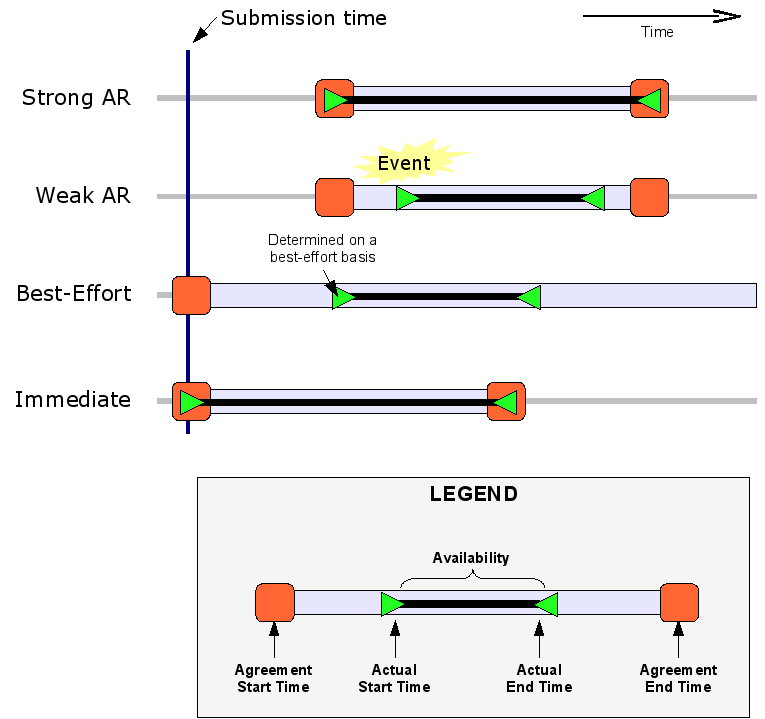
\includegraphics[width=\textwidth]{figures/availability.png}
    \caption{Availability scenarios}
    \label{fig:availability}
  \end{center}
\end{figure}

Depending on how strictly availability is defined, we encounter different \emph{availability scenarios} that can be described with terms such as `advance reservations', `batch submissions', `best--effort scheduling', etc. Since these terms tend to be highly overloaded, throughout this text we will observe the following definitions (summarized in Figure~\ref{fig:availability}):

\begin{description}
\item[Closed Advance Reservation]: Availability in this case is clearly defined \emph{in advance} with pre--agreed start and end timestamps that coincide with the start and end of the agreement. Virtual workspaces for the \emph{Virtual Labs} use case, for example, will have specific start and end times (e.g. a lab that is taught from 2pm to 4pm).
\item[Open Advance Reservation]: In event--driven applications, availability requirements are loosely defined, since the user can only specify the availability period in terms of asynchronous events (and, possibly, also a window of time during which those events are likely to arrive). However, when that event is received, availability \emph{must} be guaranteed at exactly that time, and for the duration specified. Thus, this availability scenario is an advance reservation insofar as the resource requirements are known in advance, meaning the scheduler can take steps to  provision resources preemptively in case the start event arrives, but the exact start and end times are not. The Urgent Computing use case is an example of Open AR.
\item[Best--effort Reservation]: Similarly to Open AR, this availability scenario presents loosely defined availability requirements. The user agrees to have availability defined by the resource manager, which will provision resources on a best--effort basis, taking into account local policies regarding priorities and quotas, and queueing requests if necessary. Batch jobs are an example of this availability scenario.
\item[Immediate Reservation]: In this case, availability requirements are not known until the time the resource request arrives and, once it arrives, resources must be  provisioned immediately. Unlike Open AR, the resource manager would have no way of preemptively provisioning resources for this kind of requests, and a request is rejected if resources cannot be  provisioned immediately. This scenario is, arguably, just a special case of Closed AR, where the interval between the agreement establishment time and the start time is zero.
\end{description}

In this paper we focus on Closed Advance Reservations.\footnote{Unless otherwise noted, when we refer to an \emph{advance reservation}, or an AR, we refer to a Closed Advance Reservation} We also touch upon Best--effort Reservations and, in particular, on how to schedule workloads presenting both advance reservations and best--effort reservations adequately.
